\chapter{Electron-Muon Crosscheck Studies}
\label{apx:stop:emustudies}

Our use of a dilepton control region to estimate the lost lepton
background component in Section \ref{ssec:stop:lostlep} is only useful
if the physics of $\ttbar$
processes are correctly modeled. We know from Chapter \ref{chap:afb}
that our Monte Carlo simulations do a very good job of modeling
$\ttbar$ processes on the whole, but our search for supersymmetry
demands exacting precision. For that reason, we employ a set of $e/\mu$
crosscheck regions, enriched in $\ttdilep$ and single top tW processes,
to validate the physics of our lost lepton control regions.

\subsubsection{Crosscheck Region Definitions}
\label{sssec:emu:regdefs}

We define our crosscheck regions using the following criteria:
\begin{itemize}
\item Event must pass the standard $\met$ filters.
\item Event must pass a mixed-flavor dilepton trigger (also known as
  MuonEG). The triggers we use are listed in Table
  \ref{tab:stop:trigs}.
\item We must have exactly one medium electron and one tight muon.
  \begin{itemize}
  \item The leading lepton must have $p_T >$ 30 GeV, and the
    trailing, $p_T >$ 15 GeV.
  \item The leptons must have $|\eta| <$ 2.1, and relative mini
    isolation $<$ 0.1.
  \item The leptons must have opposite charge.
  \item The dilepton invariant mass must be $>$ 20 GeV.
  \end{itemize}
\item The event must contain at least 2 jets.
\item $\met$ must be $>$ 50 GeV.
\end{itemize}
We create three regions, binned in number of b-tags: $\geq$0 tags, $\geq$1 tag,
and $\geq2$ tags. The data and Monte Carlo yields in these regions are
presented in Table \ref{tab:emu:yields}.

% E/Mu crosscheck region yields, taken from AN-16-463. Unpublished.
\begin{table}[htb]
\centering
\caption{Data and Monte Carlo yields in the $e/\mu$ crosscheck
  regions, for 35.9 fb\textsuperscript{-1}.}
\label{tab:emu:yields}
\begin{tabular}{|l|c|c|c|}

\multicolumn{4}{c}{}\\* \hline
  & $\ge0$~b-tagged~jets & $\ge1$~b-tagged~jets  & $\ge2$~b-tagged~jets \\*
Sample  & ~$\met>50$ & ~$\met>50$  & ~$\met>50$ \\*
\hline \hline

$t\bar{t}$,~$\ge2$~leptons & 123328.75 $\pm$ 106.86  & 96525.59 $\pm$ 93.60  & 35056.95 $\pm$ 55.22 \\*
$t\bar{t}$,~$1$~lepton & 1504.44 $\pm$ 13.62  & 893.81 $\pm$ 10.35  & 135.22 $\pm$ 3.92 \\*
single $t$  & 6294.76 $\pm$ 22.06  & 4358.25 $\pm$ 18.09  & 1049.82 $\pm$ 8.69 \\*
DY+Jets$\rightarrow\ell\ell$  & 2788.03 $\pm$ 265.88  & 518.67 $\pm$ 91.55  & 43.46 $\pm$ 34.35 \\*
W+Jets$\rightarrow\ell\nu$  & 315.30 $\pm$ 27.79  & 51.68 $\pm$ 10.43  & 4.91 $\pm$ 3.17 \\*
diBoson  & 1947.21 $\pm$ 19.46  & 138.08 $\pm$ 5.04  & 9.89 $\pm$ 1.31 \\*
$t\bar{t}+W$  & 223.77 $\pm$ 0.86  & 166.85 $\pm$ 0.73  & 56.97 $\pm$ 0.42 \\*
$t\bar{t}+Z$  & 232.05 $\pm$ 0.76  & 176.28 $\pm$ 0.66  & 68.44 $\pm$ 0.40 \\*
\hline \hline
All~Background  & 136634.29 $\pm$ 289.71  & 102829.20 $\pm$ 133.08  & 36425.65 $\pm$ 65.82 \\*
Data,$~ee/e\mu/\mu\mu$  & 127684.00 $\pm$ 357.33  & 96778.00 $\pm$ 311.09  & 35435.00 $\pm$ 188.24 \\*
Data/MC  & 0.93 $\pm$ 0.00  & 0.94 $\pm$ 0.00  & 0.97 $\pm$ 0.01 \\*
\hline \hline
$1$~lepton,~from~$W$  & 363.69 $\pm$ 28.00  & 72.48 $\pm$ 10.51  & 7.47 $\pm$ 3.20 \\*
$1$~lepton,~from~$t$  & 1554.12 $\pm$ 13.78  & 913.48 $\pm$ 10.43  & 137.58 $\pm$ 3.94 \\*
$\ge2$~leptons  & 134537.10 $\pm$ 288.03  & 101705.95 $\pm$ 132.26  & 36225.69 $\pm$ 65.62 \\*
$Z\rightarrow\nu\nu$  & 179.38 $\pm$ 0.73  & 137.30 $\pm$ 0.59  & 54.91 $\pm$ 0.36 \\*
\hline
\end{tabular}
\end{table}

We also check the efficiency of our $e/\mu$ triggers using a
tag-and-probe method (see Section \ref{sssec:afb:evtweights:trigeff})
in the $\met$ dataset. We measure the efficiency in both leading and
trailing lepton $p_T$, as well as overall, and find in essentially all
cases an efficiency of 0.86 $\pm$ 0.003.

\subsubsection{Kinematic Checks}
\label{sssec:emu:kinematics}

We compare the data and Monte Carlo distributions for a number of
variables in our crosscheck regions. In general, we find fairly good
agreement for number of jets, number of b-tags, jet $p_T$, and
dilepton $p_T$, as shown in Figure \ref{fig:emu:kinematics}.

% Plots of various kinematic variables, taken from AN-16-463. Unpublished.
\begin{figure}[htbp]
\centering
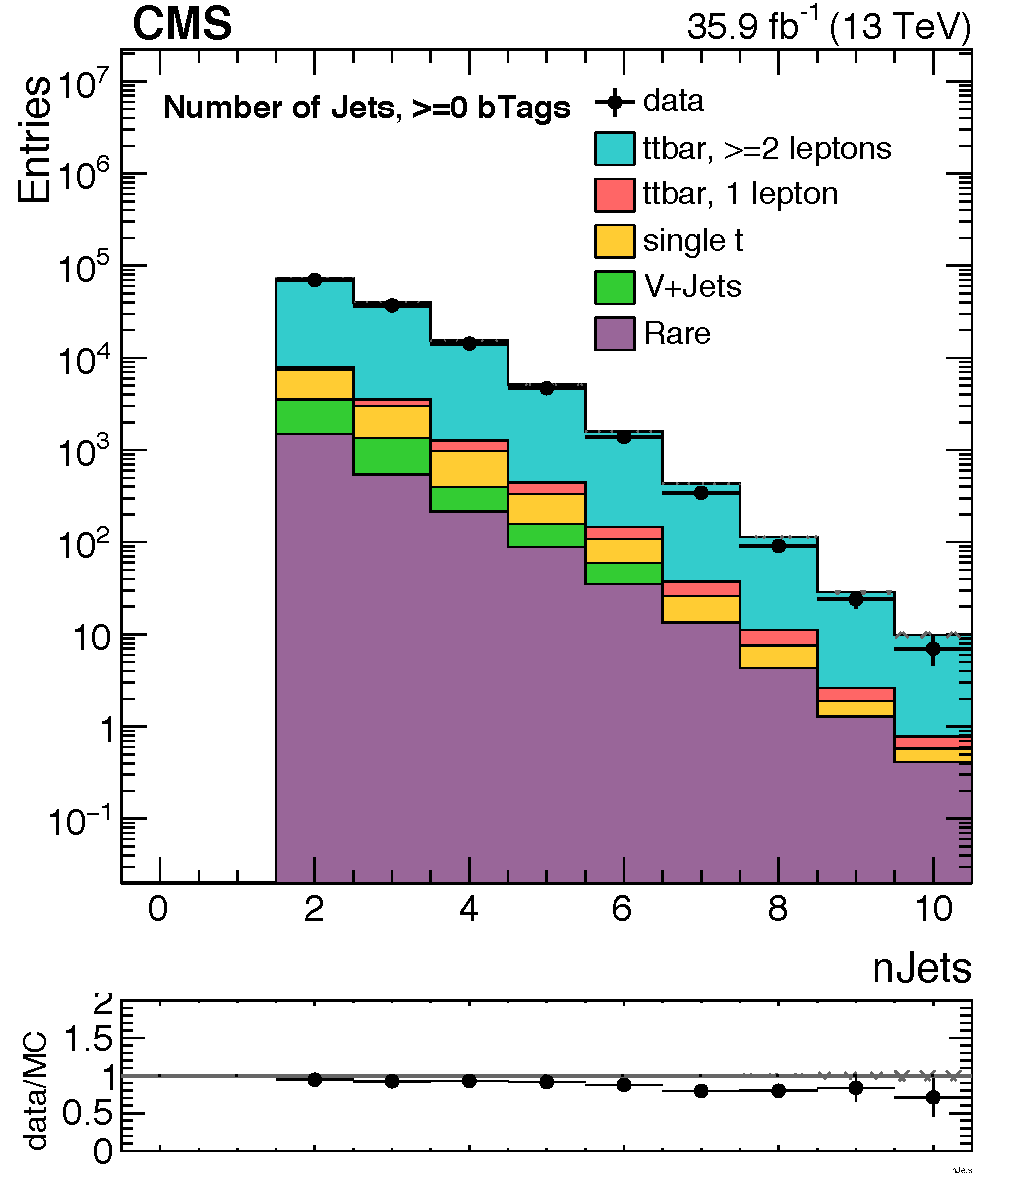
\includegraphics[width=0.45\textwidth]{figures/emuRegion_nJets.pdf}
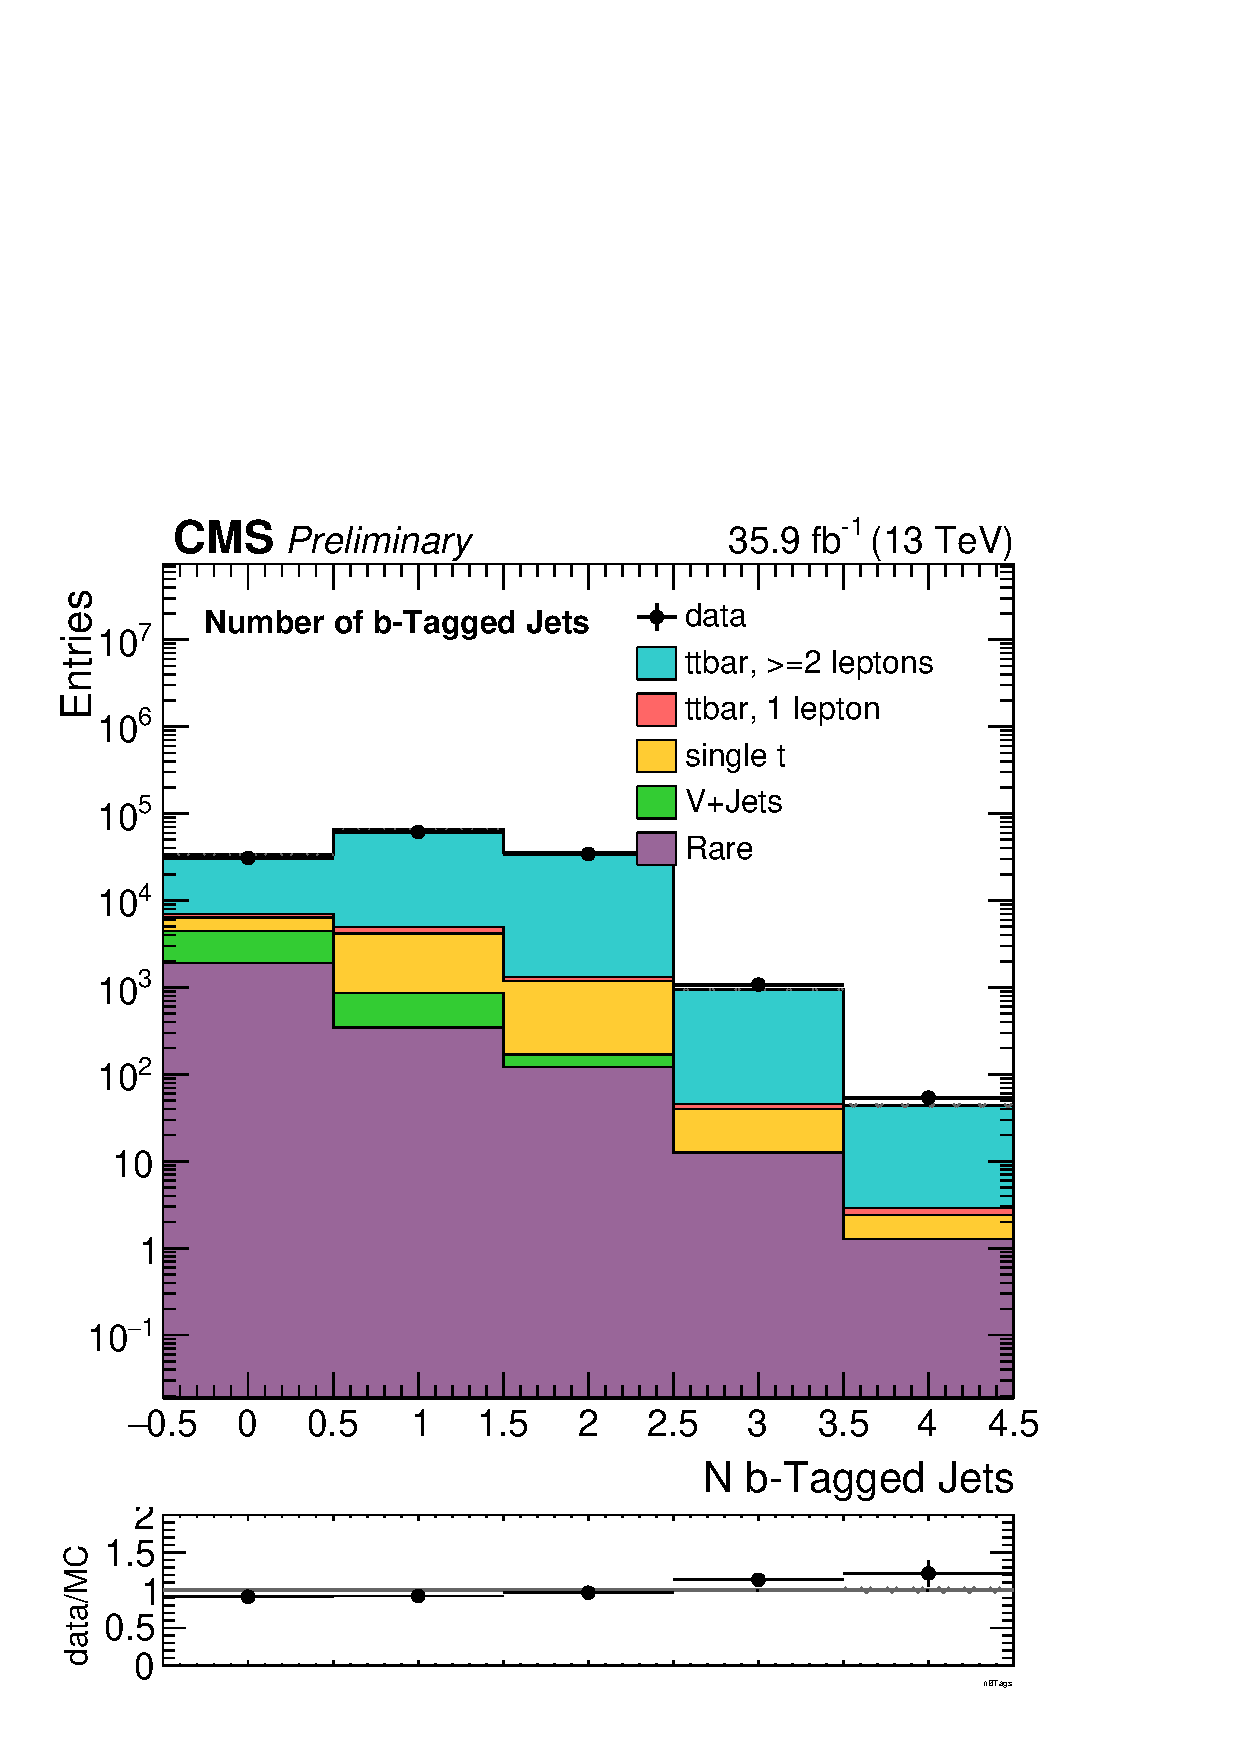
\includegraphics[width=0.45\textwidth]{figures/emuRegion_nBtags.pdf}
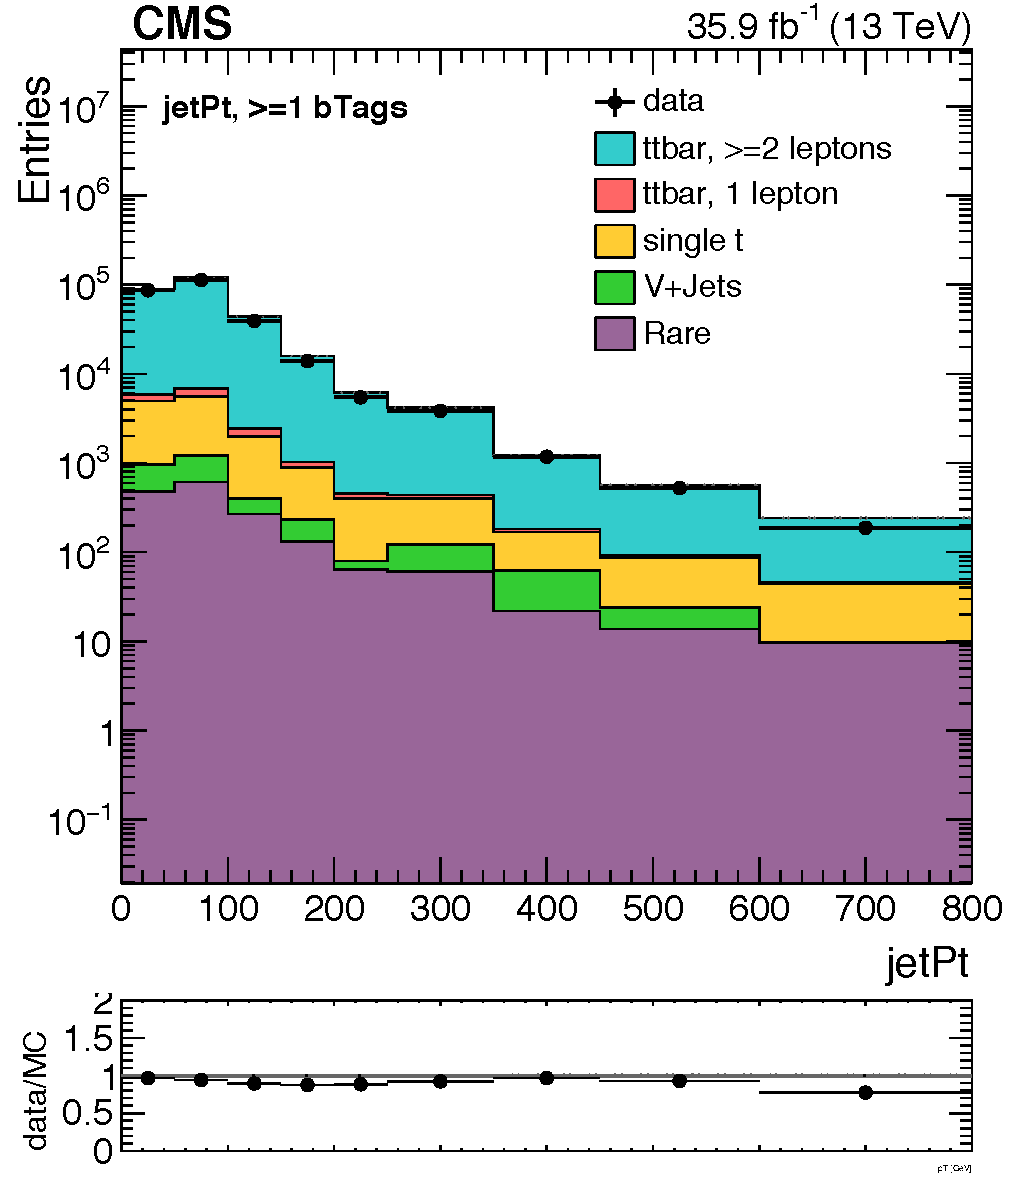
\includegraphics[width=0.45\textwidth]{figures/emuRegion_jetPt.pdf}
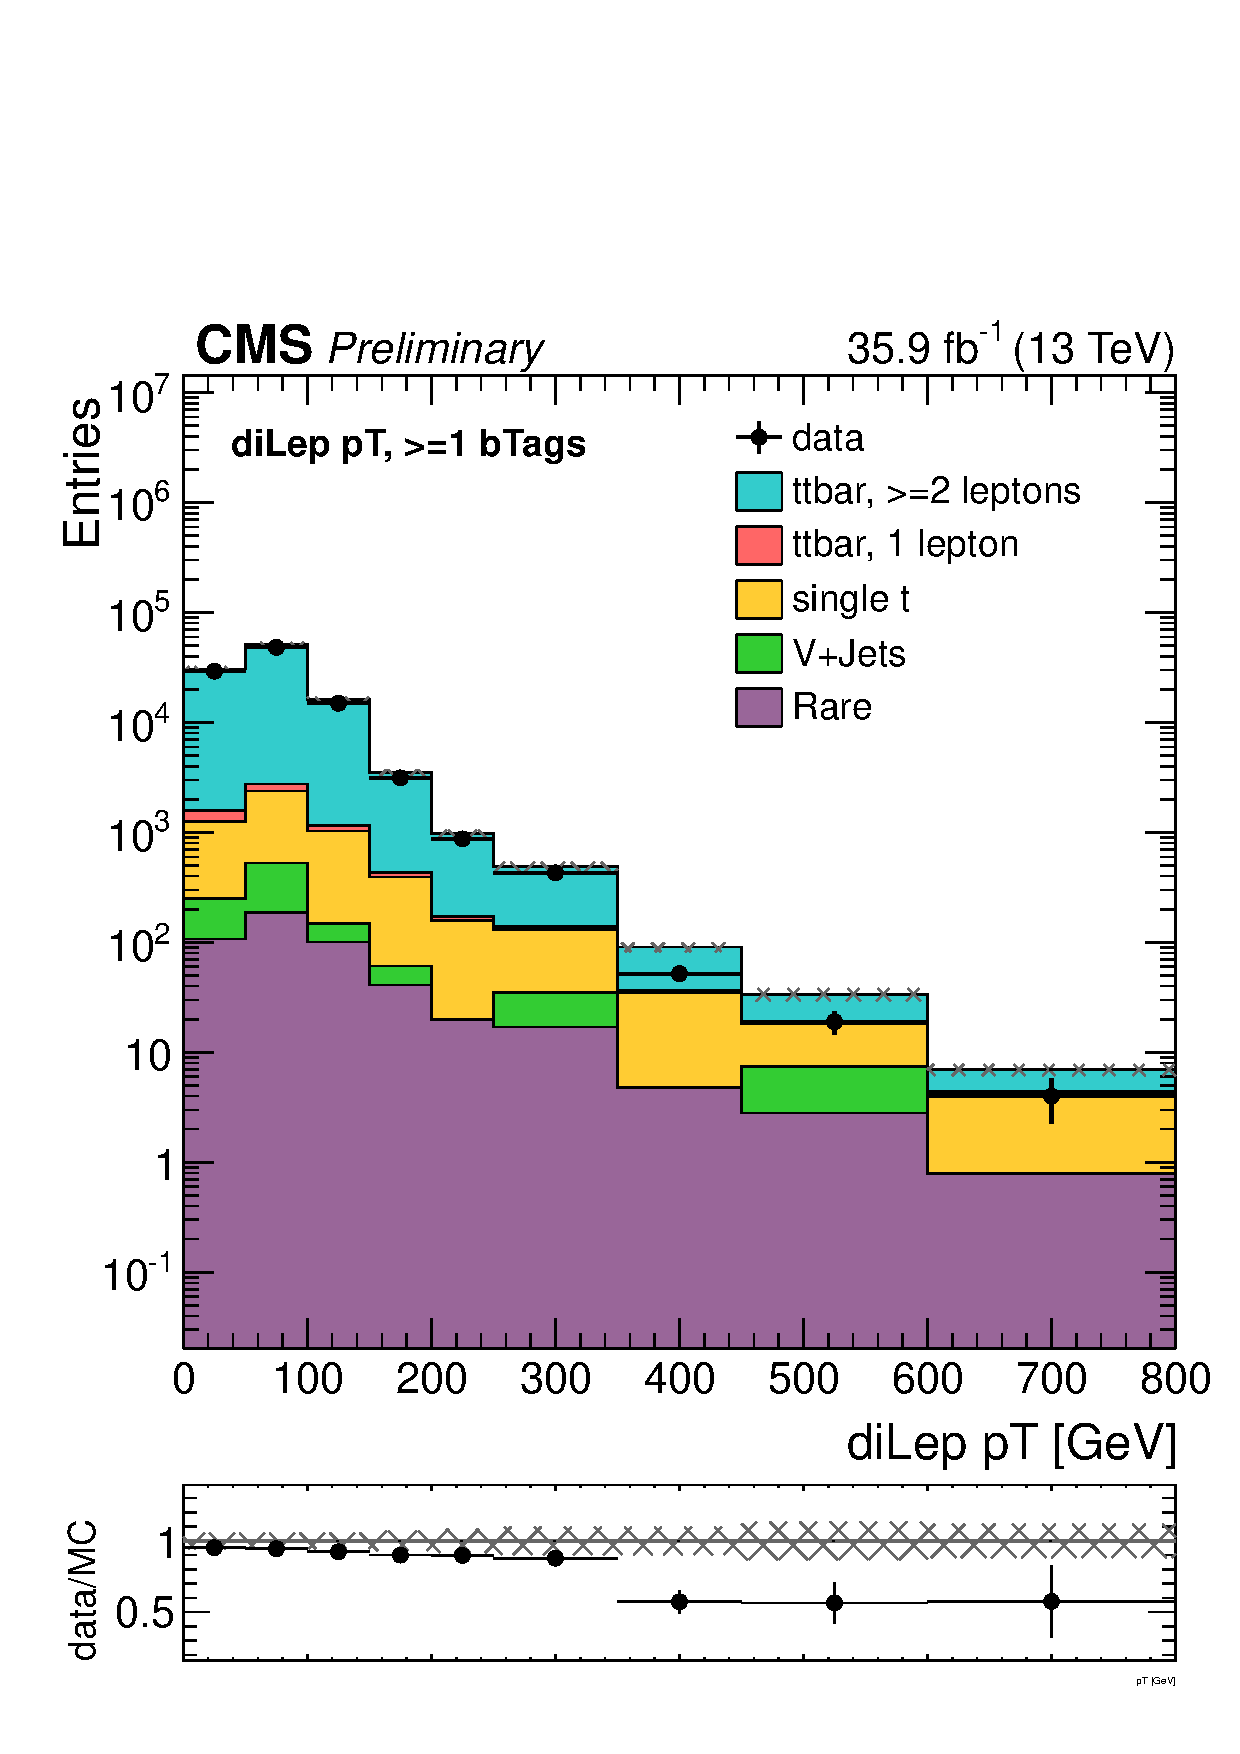
\includegraphics[width=0.45\textwidth]{figures/emuRegion_dilepPt.pdf}
\caption{Distributions of number of jets and number of b-tags in the
  $\geq$0 b-tag region, and jet $p_T$
  and dilepton $p_T$ in the $\geq$1 b-tag regions.}
\label{fig:emu:kinematics}
\end{figure}

However, the $\met$ distribution, pictured in Figure \ref{fig:emu:met}
shows significant disagreement in the last two bins. This discrepancy
must be corrected, because we perform $\met$ extrapolation in some of
our high-$\met$ control regions (see Section
\ref{sssec:stop:lostlep:estimation}, and a disagreement between data
and MC would skew our background estimate in those regions.

% MET plot taken from AN-16-463. Unpublished.
\begin{figure}[htbp]
\centering
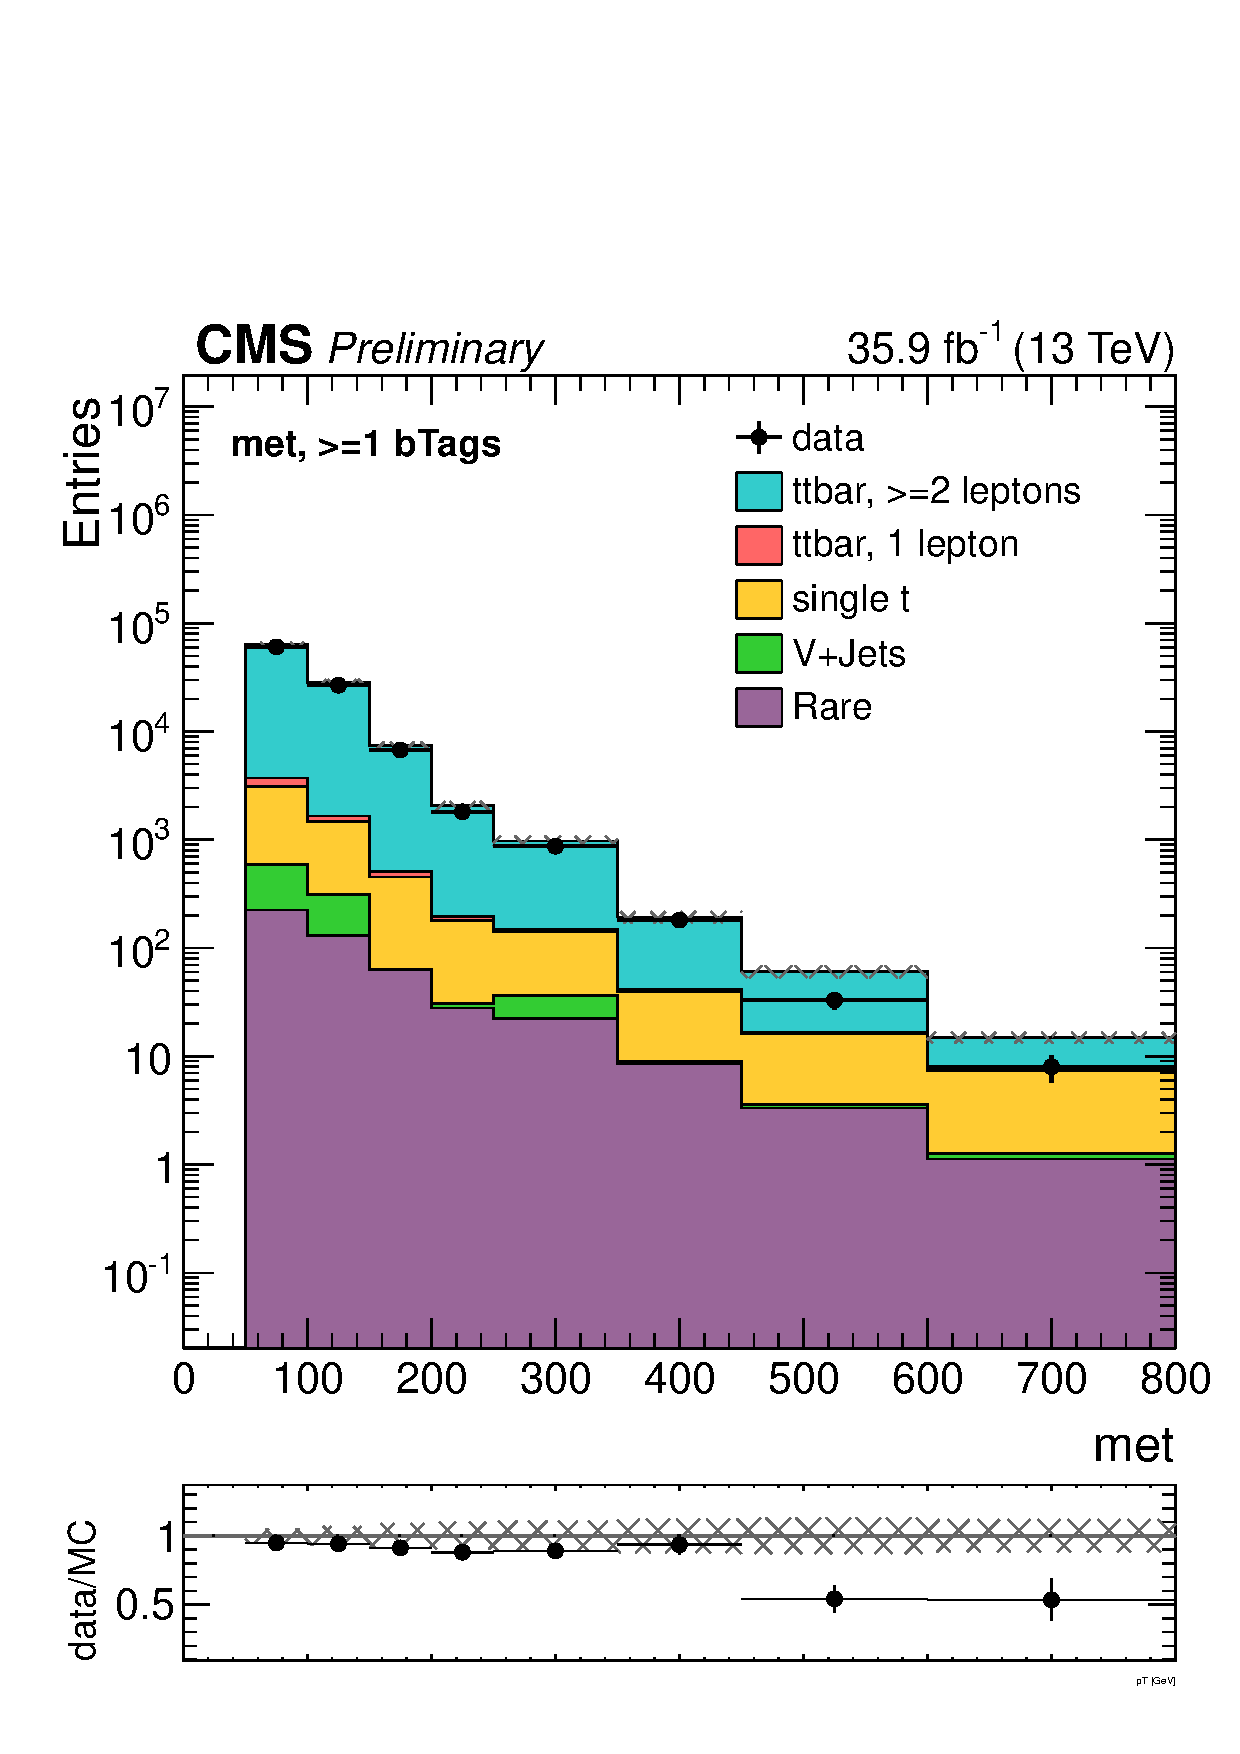
\includegraphics[width=0.6\textwidth]{figures/emuRegion_met.pdf}
\caption{Distribution of $\met$ in the $\geq$1 b-tag crosscheck
  region, showing a strong discrepancy in the last two bins.}
\label{fig:emu:met}
\end{figure}

To correct the disagreement, we calculate the data/MC ratio in each
$\met$ bin, as well as the data/MC ratio in our merged $\met$ bins
used in the extrapolation. We rescale our Monte Carlo
events so that the ratio in the individual bin equals the ratio in the
merged bin. Because we only perform $\met$ extrapolation in a few
$\met$ bins in the dilepton CRs, we only calculate and apply scale
factors to $\ttbar$ and single-top tW events that have two leptons and
that fall into one of the affected $\met$ bins. The uncertainty on the
scale factors are used to evaluate a systematic uncertainty on the
lost lepton background estimate in the bins where $\met$ extrapolation
takes place. These scale factors and their uncertainties are presented
in Table \ref{tab:emu:sfmetextrap}.

% Table of MET corrections adapted from AN-16-463. Unpublished.
\begin{table}[htb]
\centering
\caption{Data and Monte Carlo yields, and yield ratios, in our $\met$
  extrapolation regions.}
\label{tab:emu:sfmetextrap}
\begin{tabular}{|l|c|c|c|c|} \hline
Bin & Data & MC & Data/MC Norm & Scale Factor \\ \hline \hline
 \multicolumn{5}{|l|}{Region B} \\ \hline
 $450.0~<~p_{T}~<~800.0$ & $41~\pm~6.4$ & $75.9~\pm~2.5$ & $0.54~\pm~0.09$ & ---\\ \hline \hline
 $450.0~<~p_{T}~<~600.0$ & $33~\pm~5.7$ & $60.9~\pm~2.3$ & $0.54~\pm~0.09$ & $1.00~\pm~0.24$ \\ \hline
 $600.0~<~p_{T}~<~800.0$ & $8~\pm~2.8$ & $15.0~\pm~1.1$ & $0.54~\pm~0.09$ & $0.99~\pm~0.39$ \\ \hline
\hline
\multicolumn{5}{|l|}{Region E} \\ \hline
 $350.0~<~p_{T}~<~800.0$ & $222~\pm~14.9$ & $269.4~\pm~4.8$ & $0.82~\pm~0.06$ & ---\\ \hline \hline
 $350.0~<~p_{T}~<~550.0$ & $209~\pm~14.5$ & $244.1~\pm~4.5$ & $0.82~\pm~0.06$ & $1.04~\pm~0.10$ \\ \hline
 $550.0~<~p_{T}~<~800.0$ & $13~\pm~3.6$ & $25.3~\pm~1.4$ & $0.82~\pm~0.06$ & $0.62~\pm~0.18$ \\ \hline
\hline
\multicolumn{5}{|l|}{Region F, H} \\ \hline
 $250.0~<~p_{T}~<~800.0$ & $1092~\pm~33.0$ & $1246.5~\pm~14.6$ & $0.88~\pm~0.03$ & ---\\ \hline \hline
 $250.0~<~p_{T}~<~450.0$ & $1051~\pm~32.4$ & $1170.6~\pm~14.4$ & $0.88~\pm~0.03$ & $1.02~\pm~0.05$ \\ \hline
 $450.0~<~p_{T}~<~800.0$ & $41~\pm~6.4$ & $75.9~\pm~2.5$ & $0.88~\pm~0.03$ & $0.62~\pm~0.10$ \\ \hline
\end{tabular}
\end{table}

\chapter{\texorpdfstring{$\met$}{MET} Resolution Studies}
\label{apx:stop:metres}

As various sections of Chapter \ref{chap:stop} have noted, our Monte
Carlo simulations may not do a perfect job reproducing the resolution
of $\met$ reconstruction seen in actual data events. Such a shape difference has
the potential to skew several of our background estimates.
Mismodeling of the $\met$ resolution would be felt most strongly in
the lost lepton background estimate. As Section
\ref{ssec:stop:lostlep} describes, we
extrapolate from larger, merged $\met$ bins down to narrower,
individual $\met$ bins. If the $\met$ resolution is not correctly modeled,
this extrapolation may cause considerable migration of events between
$\met$ bins. In addition, $\met$ resolution effects determine how many
$\ttonelep$ events pass our $\mt$ cut, thus affecting our single
lepton from top estimate. And finally, $\met$ resolution plays an
important role in estimating our single lepton from W background,
because the W+jets process has a steeply falling $\met$ spectrum.

To correct the $\met$ resolution in our Monte Carlo simulations, and
derive systematic uncertainties on this correction, we study $\met$
resolution effects using a sample of photon+jets events. Photons are
generally well-measured within CMS. So if we treat photons as an
analogue for neutrinos, we can model $\met$ using visible particles
instead.

We begin by defining two analogous samples. As a sample of real
$\met$, we select events from $\ttonelep$ and $2\ell$ MC samples. We
require a relatively loose cut of $\met >$ 55 GeV, and accept $\geq$0
b-tags. To be our $\met$ analogues, we select $\gamma$+jets events
from simulation, as well as from data. The data are selected
from the single photon datasets listed in Table
\ref{tab:stop:datasets}, using the single photon triggers listed in
Table \ref{tab:stop:trigs}. For these photon events, we require photon $p_T
>$ 55 GeV (motivated by triggers) and exactly 0 b-tags (to remove the
influence of neutrinos produced in leptonic b-hadron decays). We
select photons using the tight photon ID provided by the EGamma POG
within CMS. We also account for trigger prescales.

From the $\ttonelep$ and $2\ell$ samples, we extract the
generator-level $p_T$ spectrum of the single or double neutrinos. We
normalize this spectrum and divide it by the normalized spectrum of
the photon $p_T$, for both photon data and MC separately. This gives
us a weighting function parameterized in $p_T$. We apply this
weighting function to the photon data and MC samples, and plot
a modified form of $\met$, defined to be the natural $\met$ in the
events added vectorially to the $p_T$ of the photon:
\begin{equation}
E_\text{T,mod}^\text{miss} = |\metvec + \vec{p}_\text{T}^\gamma|
\end{equation}

Figure \ref{fig:metres:reweighting} shows that the spectrum of
$E_\text{T,mod}^\text{miss}$ looks considerably different with and
without this reweighting to the neutrino $p_T$, indicating that the
reweighting function is far from flat. Figure
\ref{fig:metres:datamcratio} shows how the $E_\text{T,mod}^\text{miss}$
spectra compare between data and MC. Comparing the bottom ratio plots in each
case, we can see that reweighting simulation to the true $\met$
spectrum is a much larger effect than the discrepancy between data and
MC due to $\met$ resolution effects.

% Plots of reweighted and unreweighted MET-mod taken from AN-16-463. Unpublished.
\begin{figure}[htb]
\centering
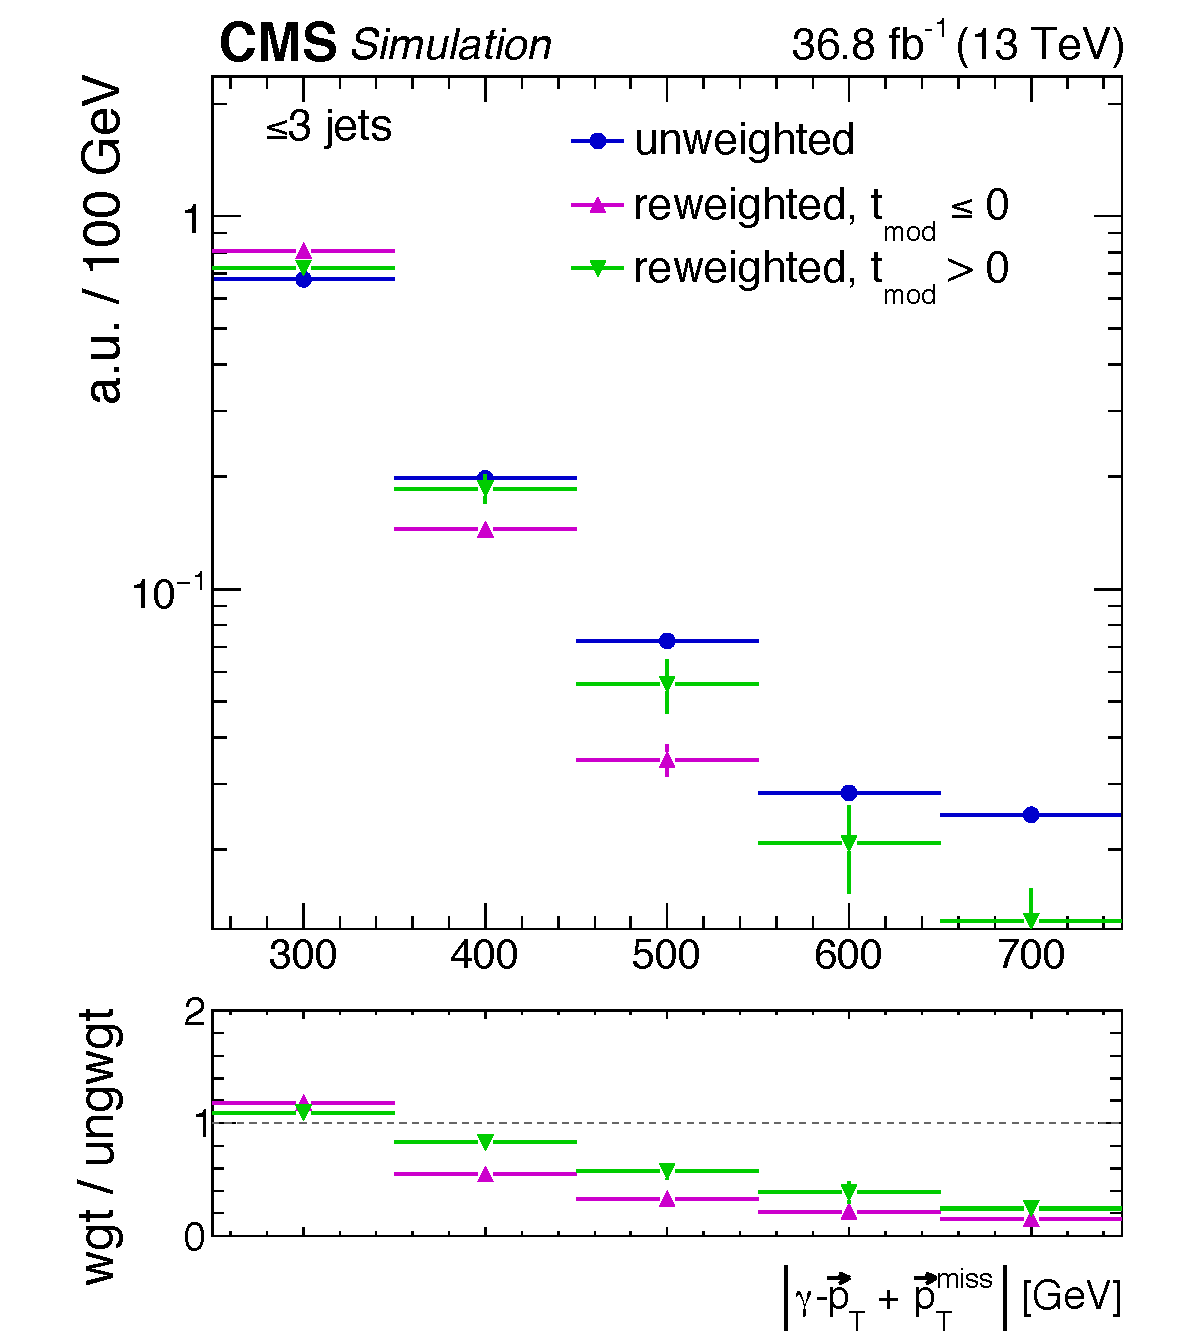
\includegraphics[width=0.325\textwidth]{figures/metres_PhotonMC_WgtVsUnwgt_AB.pdf}
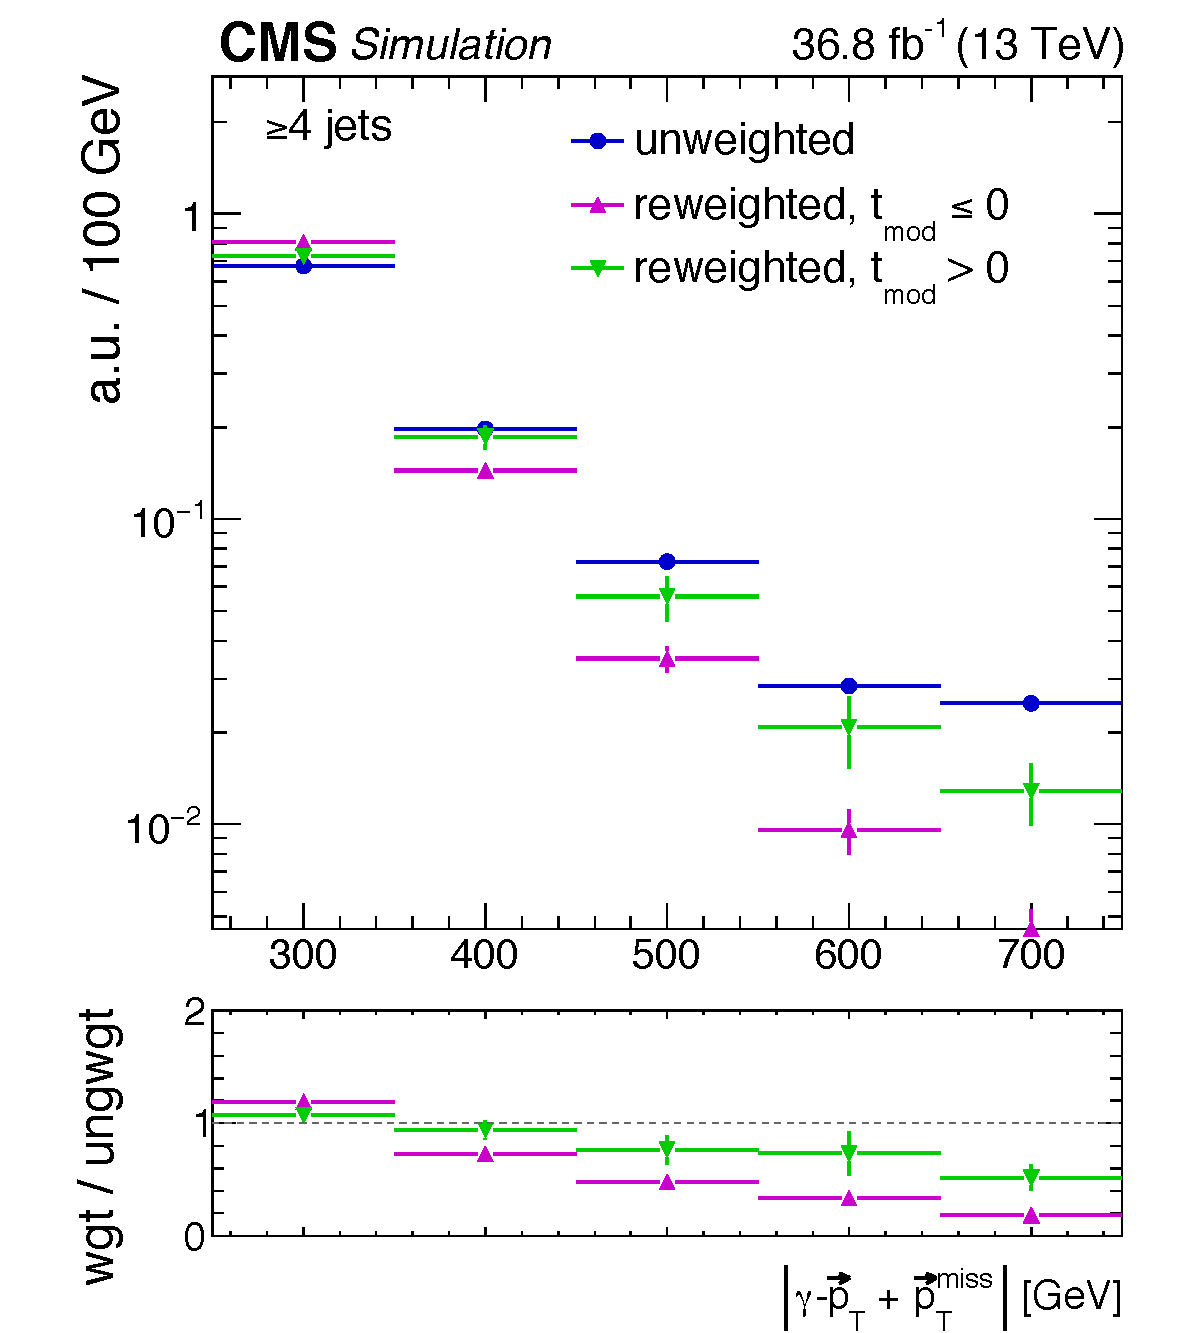
\includegraphics[width=0.325\textwidth]{figures/metres_PhotonMC_WgtVsUnwgt_CDEFGH.pdf}
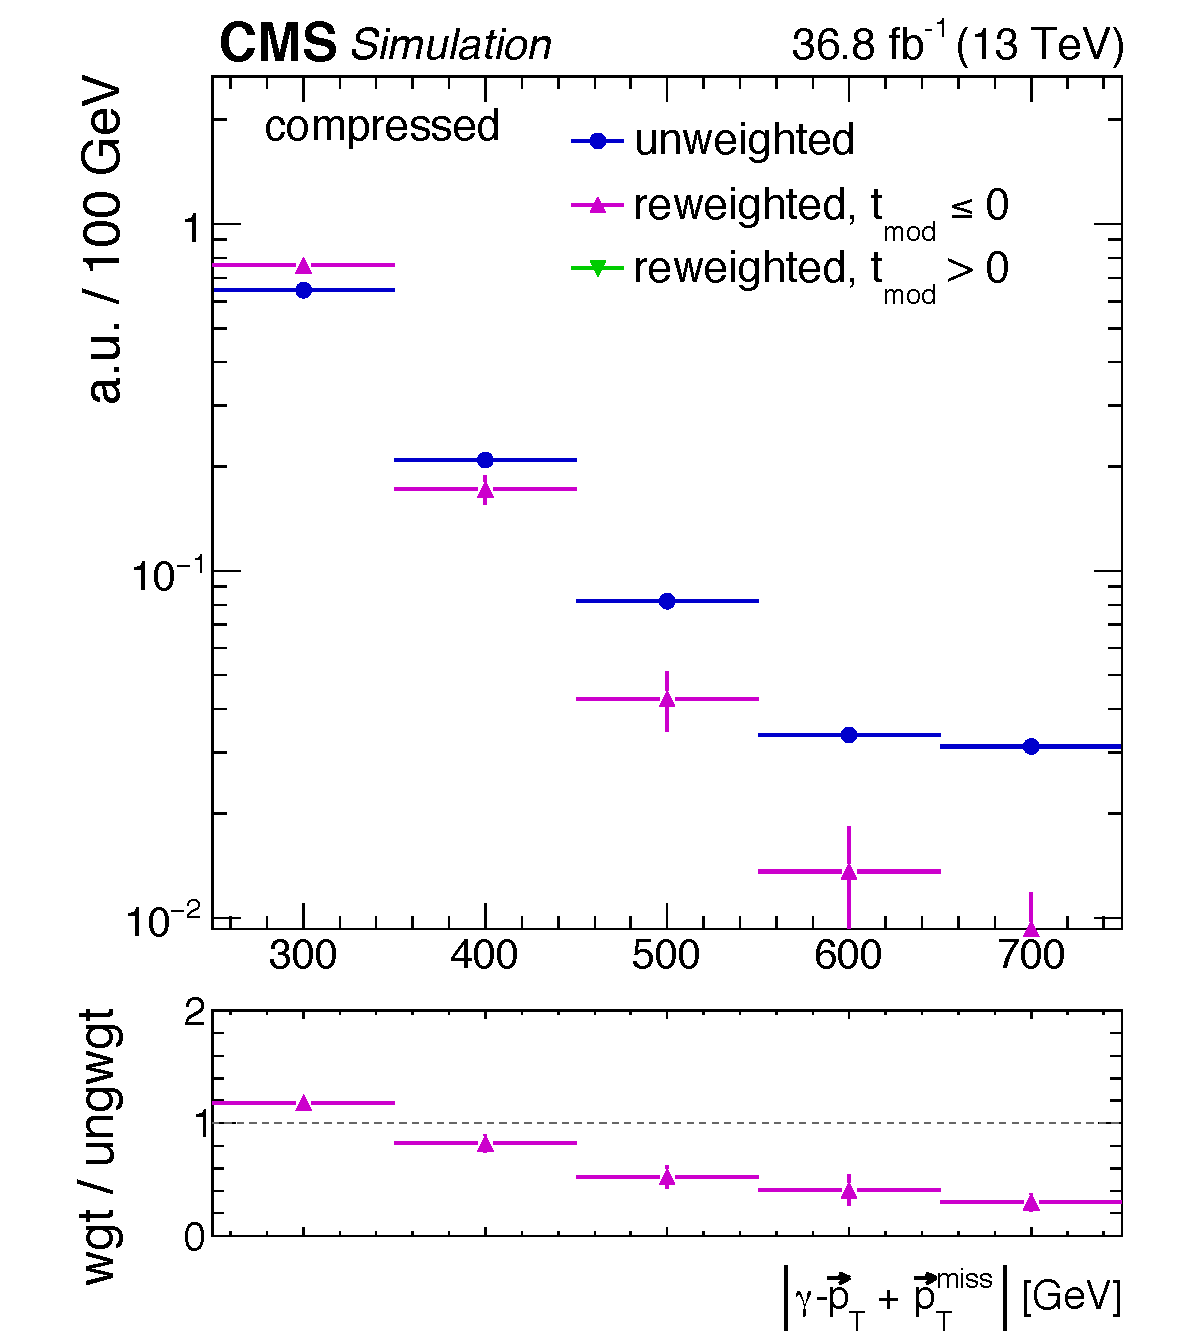
\includegraphics[width=0.325\textwidth]{figures/metres_PhotonMC_WgtVsUnwgt_I.pdf}
\caption{Normalized distributions of $E_\text{T,mod}^\text{miss}$ in
  photon MC, before and after reweighting to the $\ttbar$ neutrino $p_T$
  spectrum. The plot at left shows a 2-3 jet region, at center a
  $\geq$4 jet region, and at right a $\geq$5 jet region.}
\label{fig:metres:reweighting}
\end{figure}

% Plots of photon data and reweighted MC taken from AN-16-463. Unpublished.
% Note that these still say "Preliminary" in the header.
\begin{figure}[htb]
\centering
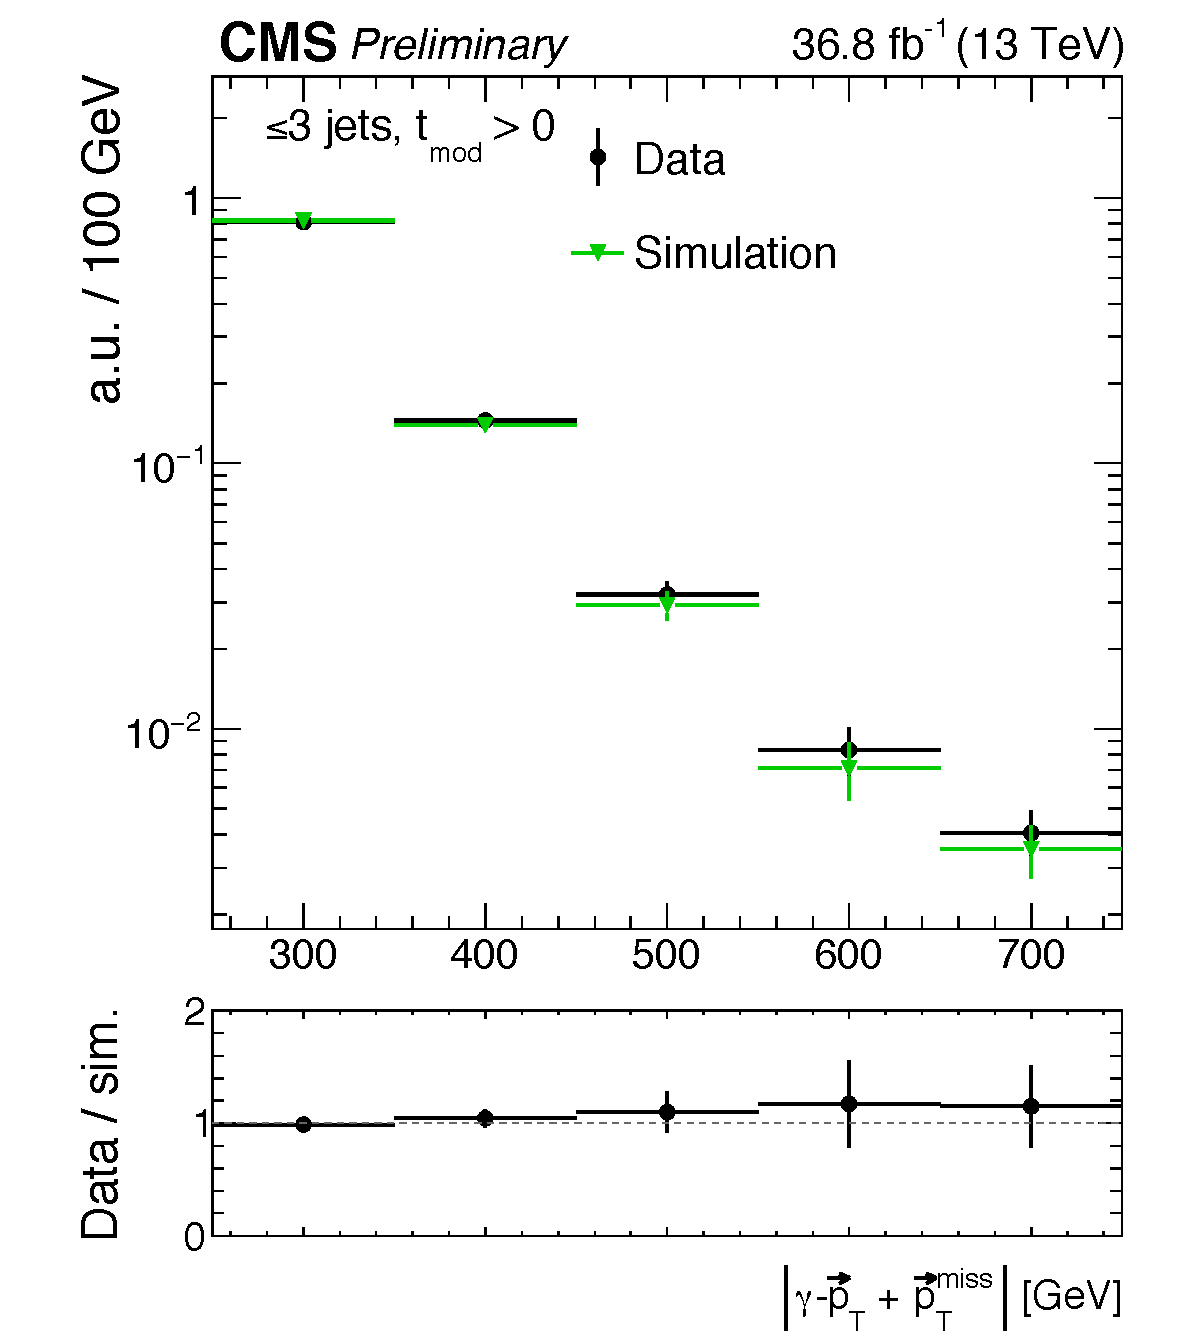
\includegraphics[width=0.245\textwidth]{figures/metres_DataVsSim_AB.pdf}
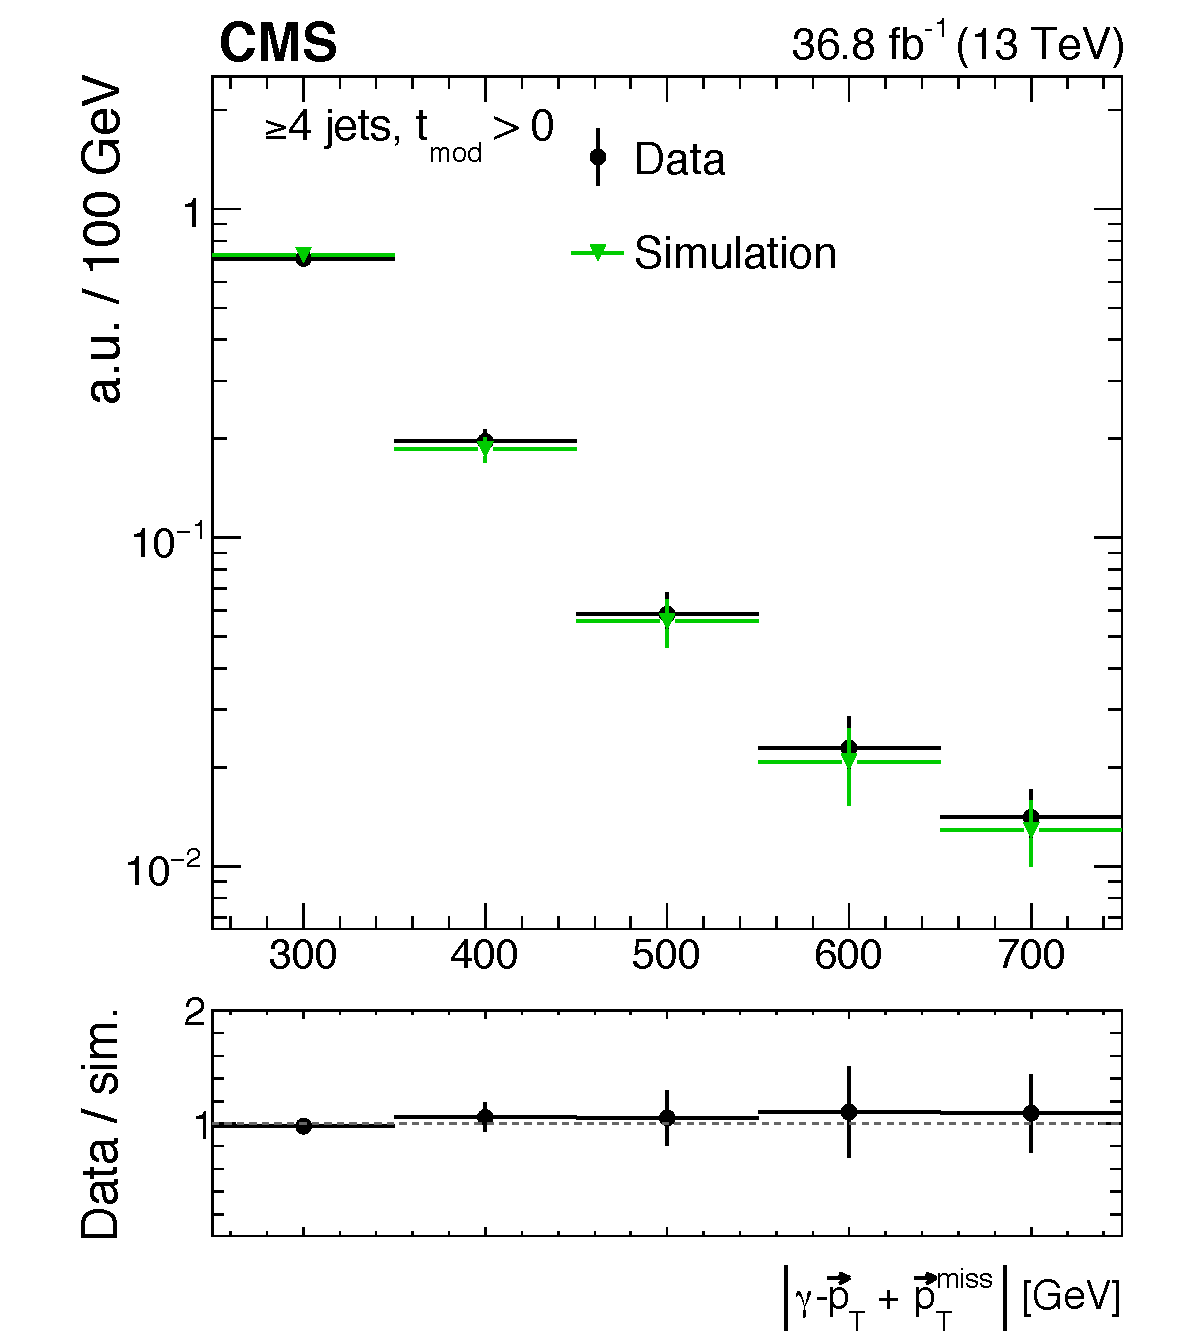
\includegraphics[width=0.245\textwidth]{figures/metres_DataVsSim_CD.pdf}
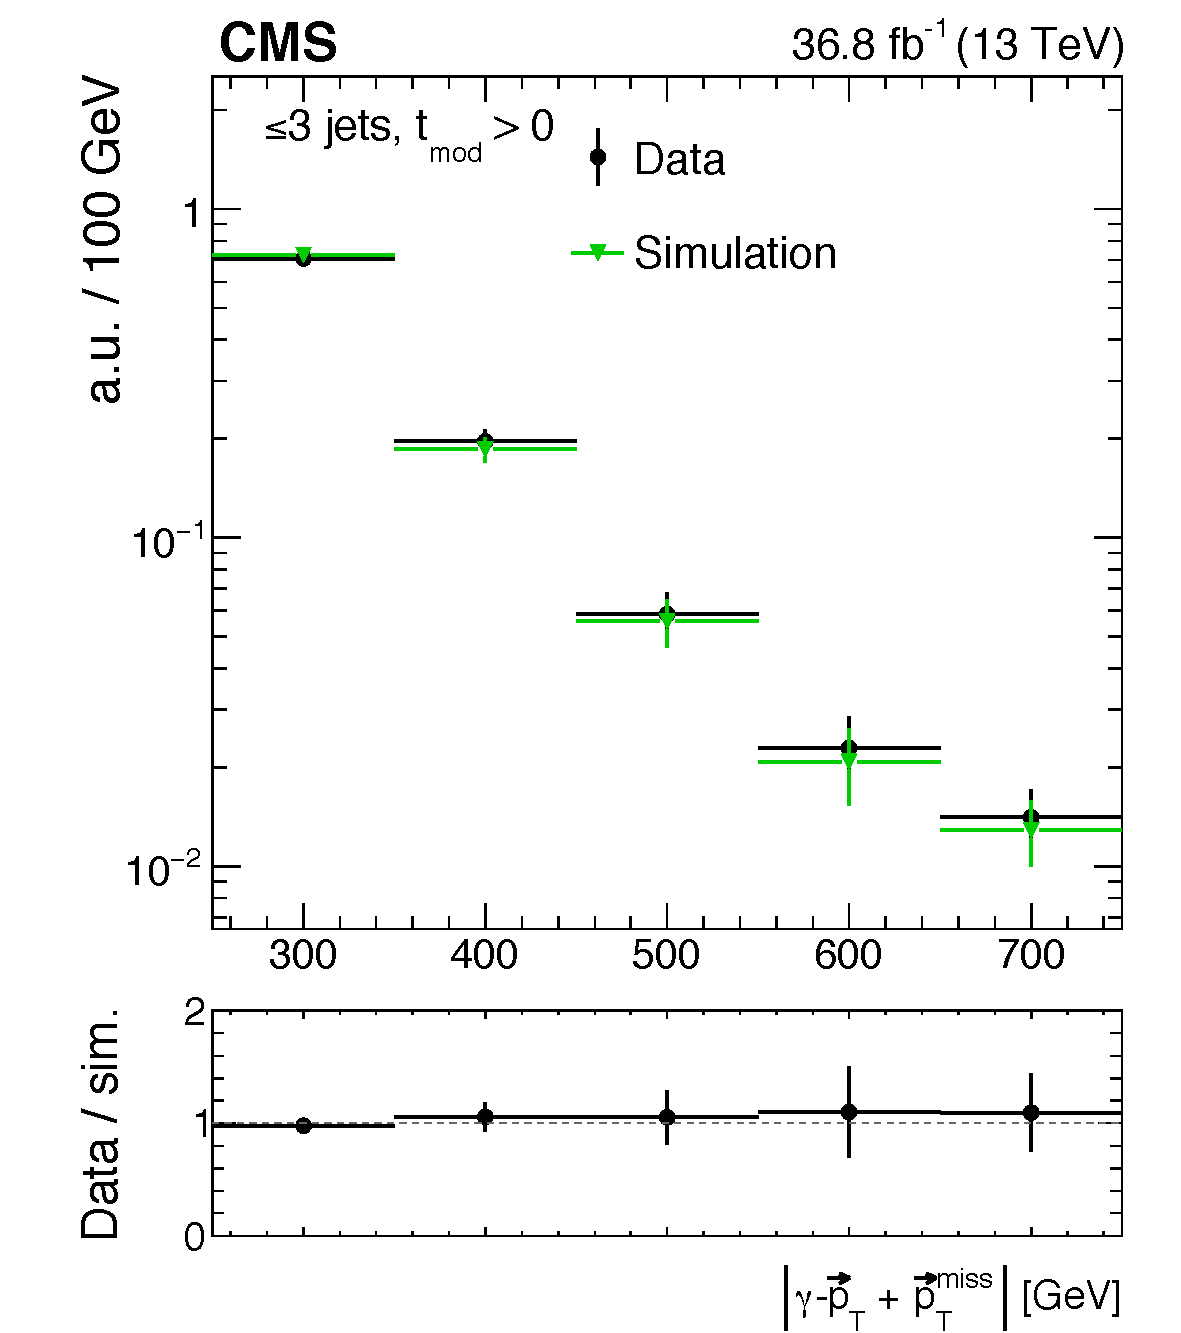
\includegraphics[width=0.245\textwidth]{figures/metres_DataVsSim_EFGH.pdf}
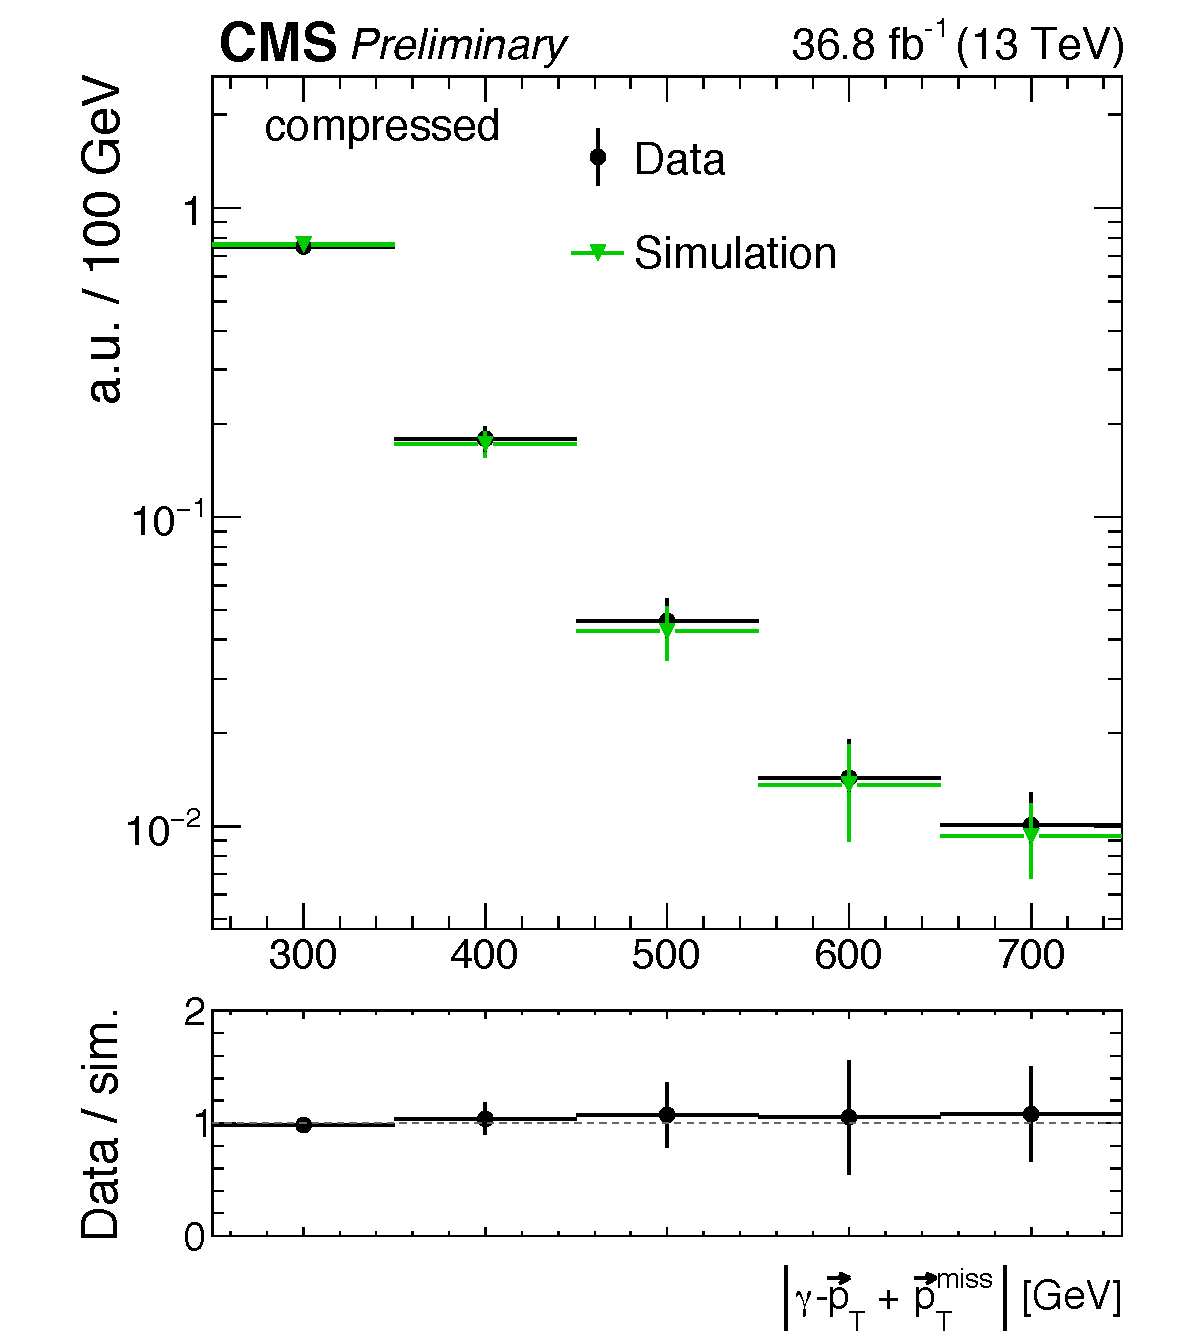
\includegraphics[width=0.245\textwidth]{figures/metres_DataVsSim_I.pdf}
\caption{Comparison of $E_\text{T,mod}^\text{miss}$ shapes in photon
  data and MC. The first plot shows a 2-3 jet region, the second shows
  $\geq$4 jets with $t_\text{mod}\leq$0, the third $geq$4 jets with
  $t_\text{mod}>$0, and the last shows a $\geq$5 jet region.}
\label{fig:metres:datamcratio}
\end{figure}

From the distributions of Figure \ref{fig:metres:datamcratio}, we
calculate the ratio of the number of events in a single $\met$ bin to
the number of events in an inclusive $\met$ bin (i.e. $\met >$ 250
GeV). We then define a $\met$ resolution scale factor, with associated
errors, equal to the bin ratio in data divided by the bin ratio in
Monte Carlo:
\begin{equation}
\text{SF}_\text{MET res.} = \frac{N_\text{bin} / N_\text{inclusive} (\text{data})}
{N_\text{bin} / N_\text{inclusive} (\text{MC})}
\end{equation}
The values and uncertainties of these scale factors in each bin are
given in Table \ref{tab:metres:scalefactors}. We apply these scale
factors to all events in the $\ttonelep$, $\ttdilep$, single top tW,
and W+Jets Monte Carlo samples. Note that because the corridor signal
regions overlap with the nominal signal regions, a single
event can take on different weights when it is considered in a nominal
SR versus in a corridor SR.

% Table of SF values made from material in AN-16-463. Unpublished.
\begin{table}[htbp]
\centering
\caption{Scale factors derived to correct $\met$ resolution for each
  of our signal regions. The uncertainties are derived from the
  statistical uncertainties on the photon data and Monte Carlo.}
\label{tab:metres:scalefactors}
\begin{tabular}{|l|c|}
\hline
Region  &  SF$_\text{MET res.}$ \\
\hline
$<4$ jets,~$\tmod \ge10$,~$\mlb<175$,~$250<\met<350$        &  0.99 $\pm$ 0.02 \\
$<4$ jets,~$\tmod \ge10$,~$\mlb<175$,~$350<\met<450$        &  1.04 $\pm$ 0.06 \\
$<4$ jets,~$\tmod \ge10$,~$\mlb<175$,~$450<\met<600$        &  1.11 $\pm$ 0.12 \\
$<4$ jets,~$\tmod \ge10$,~$\mlb<175$,~$\met>600$            &  1.17 $\pm$ 0.23 \\
\hline
$<4$ jets,~$\tmod \ge10$,~$\mlb\ge175$,~$250<\met<450$      &  1.00 $\pm$ 0.02 \\
$<4$ jets,~$\tmod \ge10$,~$\mlb\ge175$,~$450<\met<650$      &  1.11 $\pm$ 0.12 \\
$<4$ jets,~$\tmod \ge10$,~$\mlb\ge175$,~$\met>600$          &  1.17 $\pm$ 0.23 \\
\hline
$\ge4$ jets,~$\tmod <0.0$,~$\mlb<175$,~$250<\met<350$       &  0.99 $\pm$ 0.02 \\
$\ge4$ jets,~$\tmod <0.0$,~$\mlb<175$,~$350<\met<450$       &  1.05 $\pm$ 0.05 \\
$\ge4$ jets,~$\tmod <0.0$,~$\mlb<175$,~$450<\met<550$       &  1.07 $\pm$ 0.10 \\
$\ge4$ jets,~$\tmod <0.0$,~$\mlb<175$,~$550<\met<650$       &  1.10 $\pm$ 0.18 \\
$\ge4$ jets,~$\tmod <0.0$,~$\mlb<175$,~$\met>650$           &  1.14 $\pm$ 0.18 \\
\hline
$\ge4$ jets,~$\tmod <0.0$,~$\mlb\ge175$,~$250<\met<350$     &  0.99 $\pm$ 0.02 \\
$\ge4$ jets,~$\tmod <0.0$,~$\mlb\ge175$,~$350<\met<450$     &  1.05 $\pm$ 0.05 \\
$\ge4$ jets,~$\tmod <0.0$,~$\mlb\ge175$,~$450<\met<550$     &  1.07 $\pm$ 0.10 \\
$\ge4$ jets,~$\tmod <0.0$,~$\mlb\ge175$,~$\met>550$         &  1.11 $\pm$ 0.14 \\
\hline
$\ge4$ jets,~$0.0< \tmod <10$,~$\mlb<175$,~$250<\met<350$   &  0.98 $\pm$ 0.04 \\
$\ge4$ jets,~$0.0< \tmod <10$,~$\mlb<175$,~$350<\met<550$   &  1.06 $\pm$ 0.08 \\
$\ge4$ jets,~$0.0< \tmod <10$,~$\mlb<175$,~$\met>550$       &  1.10 $\pm$ 0.19 \\
\hline
$\ge4$ jets,~$0.0< \tmod <10$,~$\mlb\ge175$,~$250<\met<450$ &  0.99 $\pm$ 0.04 \\
$\ge4$ jets,~$0.0< \tmod <10$,~$\mlb\ge175$,~$\met>450$     &  1.07 $\pm$ 0.13 \\
\hline
$\ge4$ jets,~$\tmod \ge10$,~$\mlb<175$,~$250<\met<350$      &  0.98 $\pm$ 0.04 \\
$\ge4$ jets,~$\tmod \ge10$,~$\mlb<175$,~$350<\met<450$      &  1.06 $\pm$ 0.09 \\
$\ge4$ jets,~$\tmod \ge10$,~$\mlb<175$,~$450<\met<600$      &  1.07 $\pm$ 0.15 \\
$\ge4$ jets,~$\tmod \ge10$,~$\mlb<175$,~$\met>600$          &  1.08 $\pm$ 0.22 \\
\hline
$\ge4$ jets,~$\tmod \ge10$,~$\mlb\ge175$,~$250<\met<450$    &  0.99 $\pm$ 0.04 \\
$\ge4$ jets,~$\tmod \ge10$,~$\mlb\ge175$,~$\met>450$        &  1.07 $\pm$ 0.13 \\
\hline
Compressed search, $250<\met<350$                           &  0.98 $\pm$ 0.05 \\
Compressed search, $350<\met<450$                           &  1.04 $\pm$ 0.10 \\
Compressed search, $450<\met<550$                           &  1.07 $\pm$ 0.20 \\
Compressed search, $\met>550$                               &  1.07 $\pm$ 0.24 \\
\hline
\end{tabular}
\end{table}
